\section{Orçamento e viabilidade}

O sistema Smart Grid a ser implantado no campus Gama da Universidade de Brasília conta com diversos componentes eletrônicos e sistemas de software para garantir a automação do gerenciamento e produção de energia elétrica. Foram feitos os orçamentos de todos os equipamentos que irão otimizar o controle dos gastos e consumos para em seguida ser calculado a viabilidade do projeto.

\subsection{Sensores de Presença}
O sensor de presença do modelo SLEP/ST-39 custa R\$25,00 a unidade pelo fabricante Sensor Lights, contudo foi feita uma comunicação com o fornecedor e se comprado em larga escala os sensores custarão R\$20,00.

Para as salas da FGA serão utilizados 2 sensores, nos banheiros somente 1, na biblioteca 3 e na secretaria 2 sensores, onde cada um cobre uma distância de 12 metros. No prédio de aulas da FGA existem 20 salas de aulas, 6 banheiros, 1 biblioteca e uma secretaria. No RU há 2 banheiros e 6 salas de empresas, na qual cada uma delas necessita de 1 sensor, totalizando 59 sensores.

No prédio dos laboratórios e de sala de professores serão necessários 62 sensores, utilizando a mesma lógica inicial de quantidade de sensores por área. Ao total serão necessários 121 sensores, totalizando R\$2.420,00. 

\subsection{Sensores Infravermelho}
No caso do projeto Smart Grid, é necessário um par para a comunicação MESP-UAC e outro par para a comunicação UAC-UED, totalizando 4 sensores no valor total de £5.639,20 (aproximadamente R\$21.428,96) [**1**]. Os cálculos foram feitos considerando a cotação do euro no valor de R\$3,80 do dia 24/11/2016, obtido por meio da \textit{Citibank N.A}.

O sensor de comunicação infravermelho DDLS 200/200.1-10-H, fornecido pela Leuze Eletronics, utilizado para realizar a comunicação entre os prédios da FGA, custa £1.409,80 (aproximadamente R\$5.357,24) a unidade. Este sensor atua como transmissor e receptor, sendo assim necessário um par de sensores para cada par de prédios que se comunicarão.

\subsection{Sensores de Luminosidade}
A partir de análises de custos referentes à adição de elementos considerados extras ao projeto e a partir da leitura dos objetivos propostos pelo Smart Grid, que são de possibilitar uma redução efetiva do consumo de energia elétrica de forma inteligente e interativa, foi descartada a possibilidade de aferições de temperaturas por meio de sensores dedicados, tanto em condutores e quadros de distribuição, quanto em ambientes internos nas imediações da faculdade. 

Por outro lado, foi observada a possibilidade de adoção de sistemas envolvendo o controle e automação de iluminação por meio de sensores de presença e sensores fotoelétricos, tais como atuadores e dimerizadores de iluminação. Essas soluções promovem tanto a automação de sistemas externos, a partir do acionamento e desligamento de lâmpadas e refletores externos, quanto a automação interna por meio de sensores de presença e sensores fotoelétricos constituindo um sistema de dimerização automática ou apenas sistemas com acionamento e desligamento automático de lâmpadas a partir de sensores de presença.

Quanto à automação interna envolvendo sensores fotoelétricos, destacam-se os sistemas de dimerização, que são sistemas compostos por diversos componentes responsáveis por realizar dimerizações em lâmpadas fluorescentes. Esses sistemas podem ser compostos por sensores fotoelétricos interligados por sistemas de protocolo wireless, os quais, a partir de uma unidade de controle, realizarão a análise de dados, o tempo de utilização e potência fornecida pela central. Outra forma possível é a partir de um controlador central, do qual é possível retirar informações e programar a taxa e modo de dimerização requerida. Dentre as empresas que apresentam a versão pela implementação de soluções inteligentes, destacam-se a OSRAM e LUTRON. 

Dentre as soluções propostas para a automação interna, destaca-se o esquema exemplificado por componentes da empresa LUTRON, esquematizado pela Figura \ref{fig:maestrowireless}, que possuiu uma melhor viabilidade econômica em oposição às soluções completas, tais como o sistema de gerenciamento em tempo real com sistemas de interfaces gráficas, exemplificados pelo sistema QUANTUM, ilustrado pela Figura \ref{fig:sistemaquantum} [**2**]. 
\begin{figure}[!h]
	\centering
	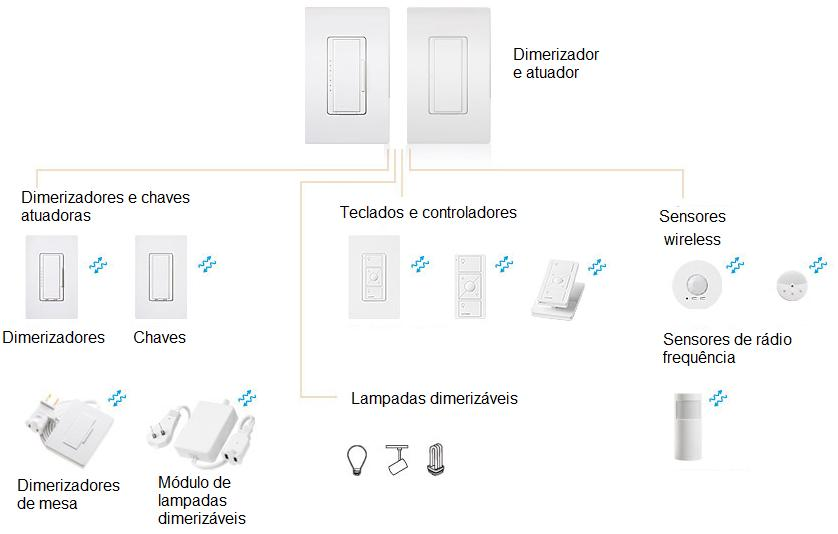
\includegraphics[width=1.0\textwidth]{figuras/maestroWireless.jpeg}
	\caption{Solução MAESTRO WIRELESS proposta por LUTRON para automação de iluminação para salas e  escritórios. Adaptado de: <http://www.lutron.com/en-US/Products/Pages/SingleRoomControls/MaestroWireless/Components.aspx>}
	\label{fig:maestrowireless}
\end{figure}

\begin{figure}[!h]
	\centering
	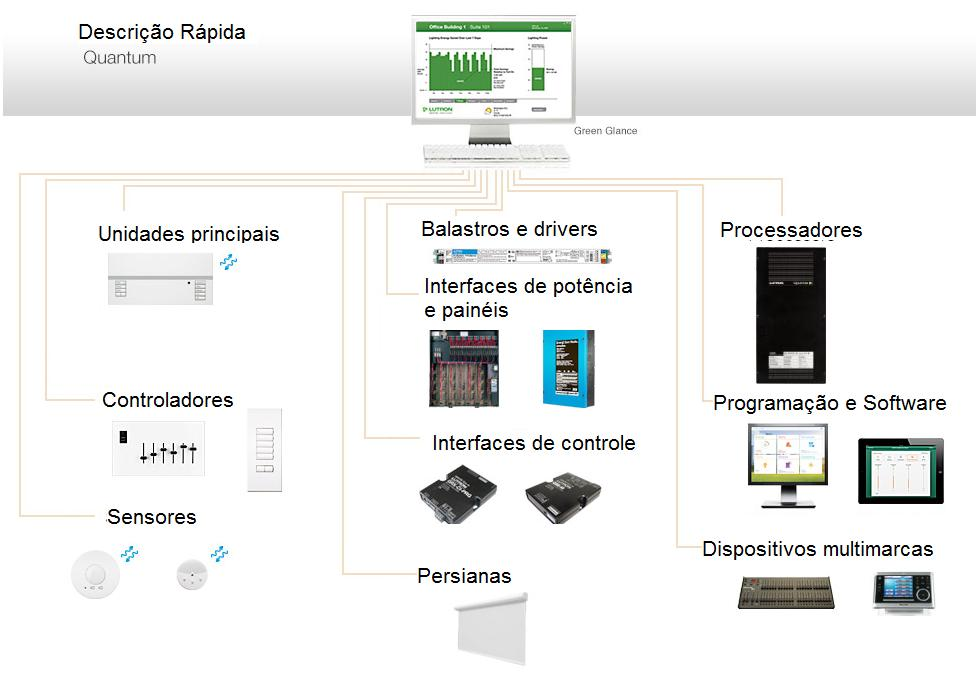
\includegraphics[width=1.0\textwidth]{figuras/sistemaQuantum.jpeg}
	\caption{Visão geral do sistema completo de automação Smart Grid (Quantum) idealizado pela empresa LUTRON}
	\label{fig:sistemaquantum}
\end{figure}

Outra solução proposta pelas empresas LUTRON [**2**] e OSRAM [**3**], os balastros de luz fluorescentes são destacados como mais rentáveis econômicamente, os quais utilizam-se de sensores/atuadores/chaves dimerizáveis para o controle ou dimerização de lampadas fluorescentes a partir desses módulos controladores (balastros). Dentre os módulos fornecidos pela empresa LUTRON, destacam-se os módulos contidos na Figura \ref{fig:tabelabalastros}.  Os módulos referentes a empresa OSRAM encontram-se na Figura \ref{fig:solucaodimerizacao} :
 
\begin{figure}[!h]
	\centering
	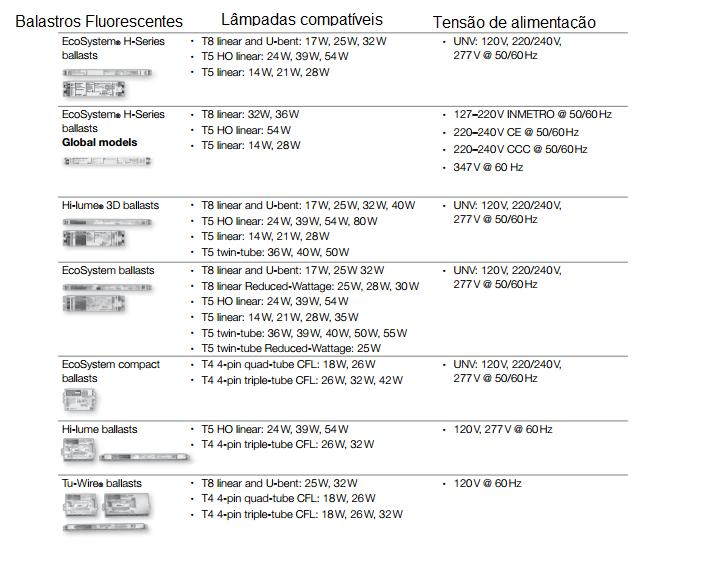
\includegraphics[width=1.0\textwidth]{figuras/tabelaBalastros.jpeg}
	\caption{Tabela comparativa entre os modelos de balastros de controle de lâmpadas fluorescentes fornecidos pela empresa LUTRON. Disponível em <www.lutron.com>, Adaptado.}
	\label{fig:tabelabalastros}
\end{figure}

\begin{figure}[!h]
	\centering
	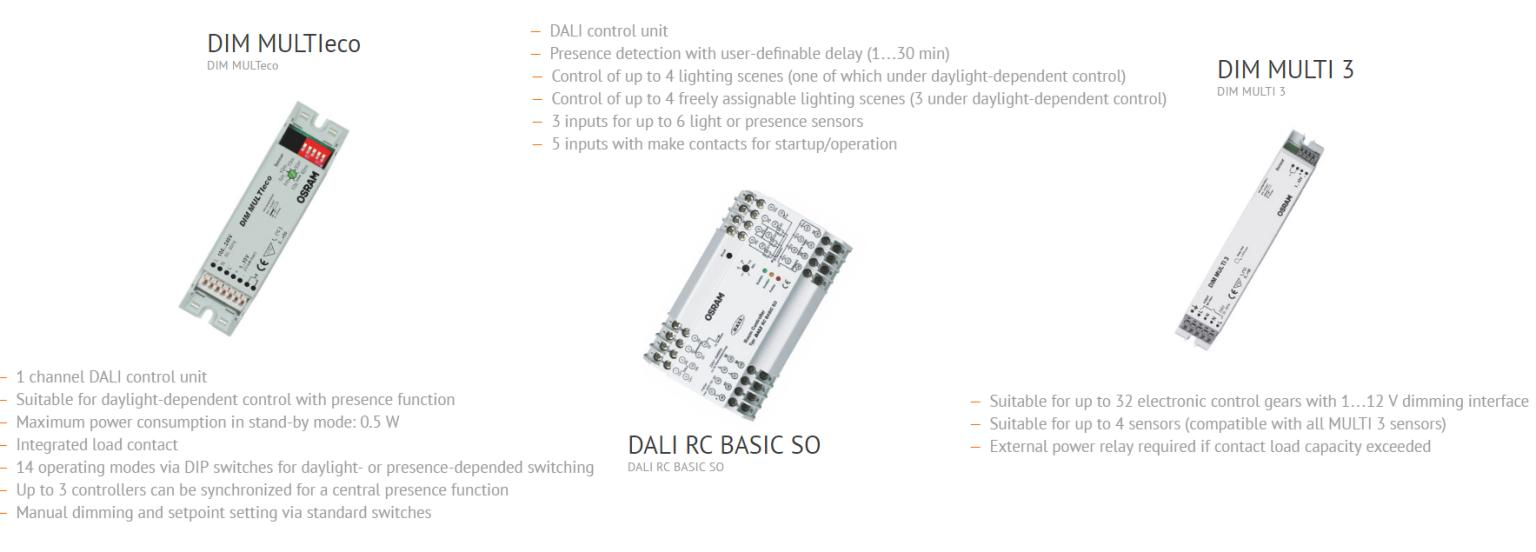
\includegraphics[width=1.0\textwidth]{figuras/solucaoDimerizacao.jpeg}
	\caption{Soluções de dimerização interna e externa, sugerida pela empresa OSRAM. Disponível em <www.osram.com> Adaptado}
	\label{fig:solucaodimerizacao}
\end{figure}

Dentre as opções mostradas na Figura \ref{fig:tabelabalastros}, a solução Hi-lume 3D apresentou-se a mais viável dentre os modelos propostos pela empresa LUTRON, por apresentar potências de trabalho maior, por ser compatível com diversos tipos de lâmpadas fluorescentes e por propiciar um espectro de dimerização de 100\% a 1\%, possibilitando maiores ganhos econômicos de energia em relação aos outros modelos propostos pela empresa. O preço unitário de unidades de Hi-lume 3D é de cerca de R\$85,00. Por outro lado, quanto às soluções propostas pela empresa OSRAM, no âmbito de balastros de dimerização, destacou-se o modelo DIM Multi 3 CONTROL, por apresentar-se como uma versão robusta, porém financeiramente rentável. Dentre as diferenças desse modelo em relação ao fornecido pela empresa LUTRON é a capacidade de fornecer e receber dados via wireless, o que facilita na integração com a análise de dados no sistema Smart Grid, fato esse que tornou possível a escolha desse produto. O preço unitário é de R\$200,00.

\subsection{Medidores Inteligentes} 
Em um sistema elétrico inteligente (Smart Grid), existe uma grande necessidade, pelo próprio conceito, da existência de um conhecimento sistemático atualizado de todo o funcionamento da rede instalada, logo é necessário implementar sensores em todos os âmbitos, de forma que se tenha a capacidade de monitorar todo o sistema. No caso do sistema instalado uma das formas de sensoriamento se baseia na instalação de medidores inteligentes de eletricidade que possibilitam conhecer tanto a utilização de eletricidade quanto a geração.

No caso em questão será instalado alguns medidores inteligentes de eletricidade, para analisar tanto a utilização de cada prédio (UED, UAC e RU) quanto a geração de eletricidade por parte da usina de biogás e pelas placas fotovoltaicas. Assim ter-se-á um medidor inteligente em cada um dos prédios de forma que seja possível saber quando e aonde está ocorrendo os maiores gastos e desperdícios de forma isolada, estes dados serão atualizados de acordo com as características do medidor. O mesmo modelo de medidor será instalado de forma tal que conheça-se a geração de eletricidade da usina de biogás e das placas fotovoltaicas sendo que ter-se-á três bancos de células.

Em última linha será instalado um medidor de tal forma que seja possível conhecer a troca de eletricidade entre a rede e o sistema elétrico interno da FGA. Assim também será possível saber de forma central aonde e quando o sistema está ou não em perfeito funcionamento, sendo possível analisar de forma remota alguns possíveis defeitos que impossibilitem o pleno funcionamento do sistema elétrico interno da FGA.

O medidor SMW 300 possui uma grande gama de funcionalidades, e por isso foi o
modelo escolhido para o projeto. Tal equipamento é trifásico, ideal para a rede da FGA, e possui as seguintes características (Manual do Usuário - SMW):
\begin{itemize}
\item Flexibilidade para mudança de tarifa convencional para tarifa branca com diferenciação tarifária;
\item Flexibilidade para mudança da comunicação (meio físico e protocolo);
\item Relé de corte e religa integrado;
\item Relógio de tempo real alimentado por bateria e supercapacitor, com monitoramento individual;
\item Memória de massa integrada para registro de até 37 dias de informações;
\item Flexibilidade de configuração dos dados a serem enviados via comunicação e apresentados no display;
\item Mecanismos de segurança para garantia de sigilo e integridade, baseado na autenticação e criptografa de dados;
\item Atualização local ou remota do firmware da metrologia ou comunicação, com implementação de segurança contra acesso mal intencionado.
\end{itemize}

O preço de cada medidor segundo simulações feitas fica em torno de R\$500,00. Tendo em vista que se pretende instalar como antes discorrido e especificado 8 medidores, tem-se que o orçamento necessário para a instalação destes fica em torno de R\$3.000,00.

\subsection{Sistema de Gerenciamento de Dados}
É de suma importância um gerenciamento de dados em um sistema inteligente de rede elétrica e para isso é necessário softwares que realizam planilhas de consumo e armazenamento de dados. A metodologia para aquisição e supervisão de dados a ser utilizado é o SCADA (\textit{Supervisory Control And Data Acquisition}), pois é o que mostra ser mais útil e eficaz atualmente [**4**]. Existem uma quantidade considerável de softwares no mercado que fazem isso. Esses softwares administram os dados coletados e apresentam em forma de gráficos para uma melhor visualização. Esses também tem ferramentas de cálculos estatísticos para a análise dos dados coletados [**5**].

A solução encontrada foi do uso do software SCADA Action.NET que faz a aquisição de dados e controle de supervisão do processo controlado. Esse trabalha em plataforma de 64 bits, que suporta todos os protocolos da área elétrica, o que anula o risco de não compatibilidade entre os dispositivos da automação [**6**].

O fornecedor do software escolhido para uma estimativa de custos do projeto foi a Spin Engenharia de automação. Este fornece o software Action.NET e seu preço varia de acordo com que o software trabalhará e suas funcionalidades.

Como o produto desejado não é algo que é vendido em prateleiras, ou seja, é comercializado para empresas e não consumidores comuns, a disponibilização de preços por parte das empresas não é simples. Como não houve resposta da empresa, utilizou os dados fornecidos pela empresa LABVIEW de um software semelhante ao desejado. O preço obtido foi de R\$45.250,00 [**7**].

\subsection{Central de Gerenciamento de Dados}
É necessário haver um espaço para ser a sede do gerenciamento dos dados obtidos por todo o sistema Smart Grid. Nessa central serão analisados os insumos adquiridos pelo software SCADA, onde os técnicos e responsáveis poderão trabalhar de forma confortável e adequada para interpretar os resultados e tomar as decisões necessárias. 

Será adquirido um contêiner para montar uma central de monitoramento de todo o sistema Smart Grid. O tamanho é o mesmo dos containers já usados na FGA e supre as necessidades ideais do projeto, possuindo um acabamento superior, com montagem em layouts específicos de acordo com a necessidade do projeto, módulos acopláveis permitindo a construção de ambientes amplos e conforto térmico superior, pois todas as paredes são feitas de termopainel [**8**]. 

Nesta central de monitoramento, é necessário haver uma máquina a qual será instalada o software e todo o trabalho será feito. O equipamento escolhido foi o Workstation da Dell T5810 que é ideal para efetuar esse tipo de monitoramento com o software SCADA que foi o escolhido. O computador seria usado para análises de dados do consumo de energia nos vários prédios da FGA, plotagem de gráficos e emissões de relatórios com tudo isso feito pelo software [**9**].

\subsection{Gerador Biogás}
Para a geração de energia a partir do biogás o gerador escolhido foi o BAT 5000 Bio, por possuir uma boa taxa de consumo do biogás gerado, para a conversão para energia elétrica. O gerador foi encontrado na empresa Senergam – Soluções Energéticas e Ambientas, e tem seu valor de R\$4.700,00 [**10**].

\subsection{Quadro de Transferência Automática}
O Quadro de transferência automática escolhido fora o Strazmaq, Modelo QTASTZ-MONO-8K-30A, devido sua compatibilidade com o gerador que gera uma potência aparente de 4 KVA, sendo que o quadro suporta até 8 KVA. Ele também possui a possibilidade de programação de funcionamento, gerando uma maior flexibilidade ao usuário, já que ele pode controlar o gerador. O quadro de transferência automático citado foi encontrado na empresa S\&S Grupo Geradores, pelo preço de R\$2.658,00 [**11**].
\begin{figure}[!h]
	\centering
	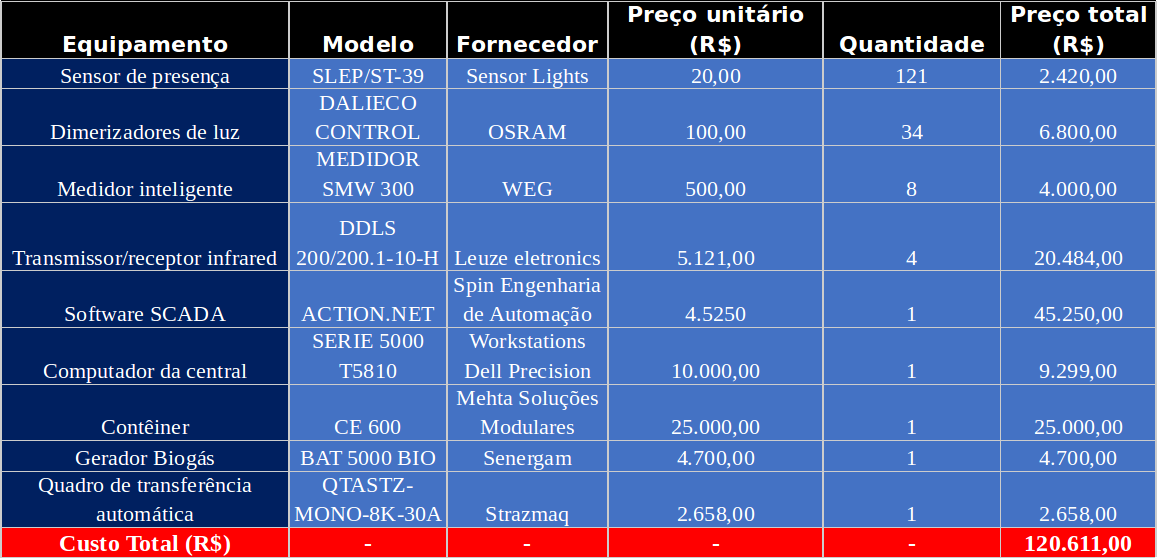
\includegraphics[width=1.0\textwidth]{figuras/tabelaCustosFinal.png}
	\caption{Tabela final de custos do sistema de automatização da Faculdade Gama/UnB}
	\label{fig:tabelacustosfinais}
\end{figure}








\begin{comment}
[1] http://www.bsaswiss.ch/ddls-200200.1-10-h-257133C653_EURENG.phtm
[2] http://www.lutron.com/TechnicalDocumentLibrary/Hi-lume3D%20rev%20b.pdf 
[3] https://dsoem.osram.com/products/led-technology/light-management-systems/dalieco/controllers/dalieco-control/dalieco-control/ 
[4] Instrumatic, Sistemas de Supervisão e aquisição de dados, 2011. Disponível em: <http://www.instrumatic.com.br/artigo/sistemas-de-supervisao-e-aquisicao-de-dados>. Acesso em: 23 de outubro de 2016.
[5] B-Scada®, Enterprise ESCADA. Disponivel em <http://www.scada.com/pt-PT/Software/enterprise-scada>. Acesso em: 30 de outubro de 2016.
[6] http://spinengenharia.com.br/produtos/action-net/
[7] http://www.ni.com/labview/buy/pt/
[8] http://veiculo.mercadolivre.com.br/MLB-813973893-venda-e-locaco-de-container-habitavel-de-alto-padro-_JM#redirectedFromParent
[9] http://www.dell.com/br/empresa/p/precision-t5810- workstation/pd?oc=cup5810w7pbr&ref=PD_OC

[10] http://www.senergam.com.br/pagina/detalhes/8/Gerador-De-Energia-Eletrica-A-Biogas.html

[11] http://www.lojassgeradores.com.br/geradores-de-energia/quadro-de-transferencia-automatica-qta/quadro-de-transferencia-automatica-qta-monofasico-12-kva-30-a-strazmaq
\end{comment}